\chapter{map objects}
\label{map} \index{Map object}

The main purpose of {\em map objects} is to provide functionality for handling and storing spatial information in terms of geographical maps. In addition, {\em map objects} serve as auxiliary objects for regression models with spatial effects, where the effect of a location variable is to be included via a spatially correlated prior. In this context, {\em map objects} store the neighborhood structure of a map and provide functionality to compute weights associated with this neighborhood structure.

The typical approach will be as follows: A {\em map object} is created, the boundary information of a geographical map is read from an external file and stored in the {\em map object}. This can be achieved using the #infile# command, see
\autoref{mapinfile} below. Based on the boundary information, the {\em map object} automatically computes the neighborhood
structure of the map and the weights associated with the neighborhood structure. Since there are several proposals in the
spatial statistics literature for defining weights, the user is given the choice between a couple of alternatives.  Afterwards, the {\em map object} can be passed to the regression function of a regression object to estimate regression models with spatial covariates, see \autoref{XXX}.

Note that \BayesX itself offers only limited functionality for creating and/or modifying geographical information. The {\it R2BayesX} R package provides some functionality for creating and manipulating boundary information and for storing it in file formats that can be processed by \BayesX.

\section{Method infile}
 \label{mapinfile} 
 \index{Map object!Infile command} 
 \index{Map object!Boundary files} 
 \index{Boundary files} 
 \index{Graph files}
 \index{Reading graph files} 
 \index{Reading boundary files}

\subsection{Description}

Method #infile# is used to read the boundary information of a geographical map stored in an external file. Currently, two file formats are supported: {\em boundary files} and {\em graph files}. A {\em boundary file} contains information about the boundaries of the different regions of a map in terms of closed polygons, i.e. the boundary of each region is represented by a set of connected straight lines. A detailed description of the structure of boundary files is given below.

A {\em graph file} stores the nodes and edges of a graph representing the neighborhood structure of a map. In addition,
weights associated with the edges of the graph can be specified. In terms of geographical maps, the nodes of the graph correspond to the different regions while the edges specify the neighborhood structure. As a consequence, the neighborhood structure of a geographical map is immediately available in a {\em graph file} while it has to be computed from the polygons in case of a {\em boundary file} (a task which may be time-consuming). Therefore an advisable strategy is to read a {\em boundary files} only once to compute the neighborhood structure and to store it as a {\em graph file} afterwards (using the #outfile# command, see \autoref{mapoutfile}). This is particularly the case for geographical maps with a lot of regions or very detailed representation of the polygon shapes. However, using {\em graph files} also has a disadvantage: Visualization of geographical information is only possible with boundary files since only these contain the information on the boundaries required for visual representation.

\subsection{Syntax}

#> #{\em objectname}.#infile# [{\em , options}] #using# {\em filename}

Method #infile# reads the map information stored in the {\em boundary} or {\em graph file} {\em filename}. If option #graph# is specified, \BayesX expects a {\em graph file}, otherwise a {\em boundary file} is expected.

\subsubsection*{Structure of a Boundary File}

A {\em boundary file} provides the boundary information of a geographical map in terms of closed polygons. For each region of the map, the boundary files contains a block of lines defining the name of the region, the number of lines the polygon consists of, and the polygons themselves. The first line of such a block contains the region code surrounded by quotation marks and the number of lines the polygon of the region consists of. The region code and the number of lines must be separated by a comma. The subsequent lines contain the coordinates of the straight lines that form the boundary of the region. The straight lines are represented by the coordinates of their end points. Coordinates must be separated by a comma.

To give an example we print a (small) part of the {\em boundary file} of Germany:

\begin{multicols}{3}
\footnotesize

\hspace{1cm}  $\vdots$

"6634",31 \\
2319.26831,4344.48828 \\
2375.45435,4399.50391 \\
2390.67139,4446.32520 \\
2470.26807,4405.35645 \\
2576.78735,4379.60449 \\
2607.22144,4337.46533 \\
2627.12061,4356.19385 \\
2662.23682,4355.02344 \\
2691.50024,4311.71338 \\
2726.61646,4310.54248 \\
2716.08154,4256.69775 \\
2710.22900,4227.43408 \\
2680.96533,4234.45752 \\
2583.81055,4165.39551 \\
2568.59351,4096.33398 \\
2520.60132,4042.48901 \\
2535.81836,3941.82251 \\
2490.16724,3920.75269 \\
2451.53955,3903.19458 \\
2437.49292,3924.26440 \\
2369.60156,3933.62866 \\
2359.06665,3951.18677 \\
2285.32275,3969.91553 \\
2258.40015,4061.21753 \\
2197.53223,4049.51221 \\
2162.41602,4086.96948 \\
2204.55542,4091.65161 \\
2192.85010,4125.59717 \\
2284.15210,4220.41113 \\
2339.16748,4292.98438 \\
2319.26831,4344.48828

\hspace{1cm} $\vdots$

\end{multicols}
\normalsize

\vspace{0.3cm}

The  map corresponding to this part of the {\em boundary file} can be found in \autoref{partgermany}. Note that the first and the last point of a polygon must be identical (see the example above) to obtain a closed polygon.


\begin{figure}[ht]
\centering
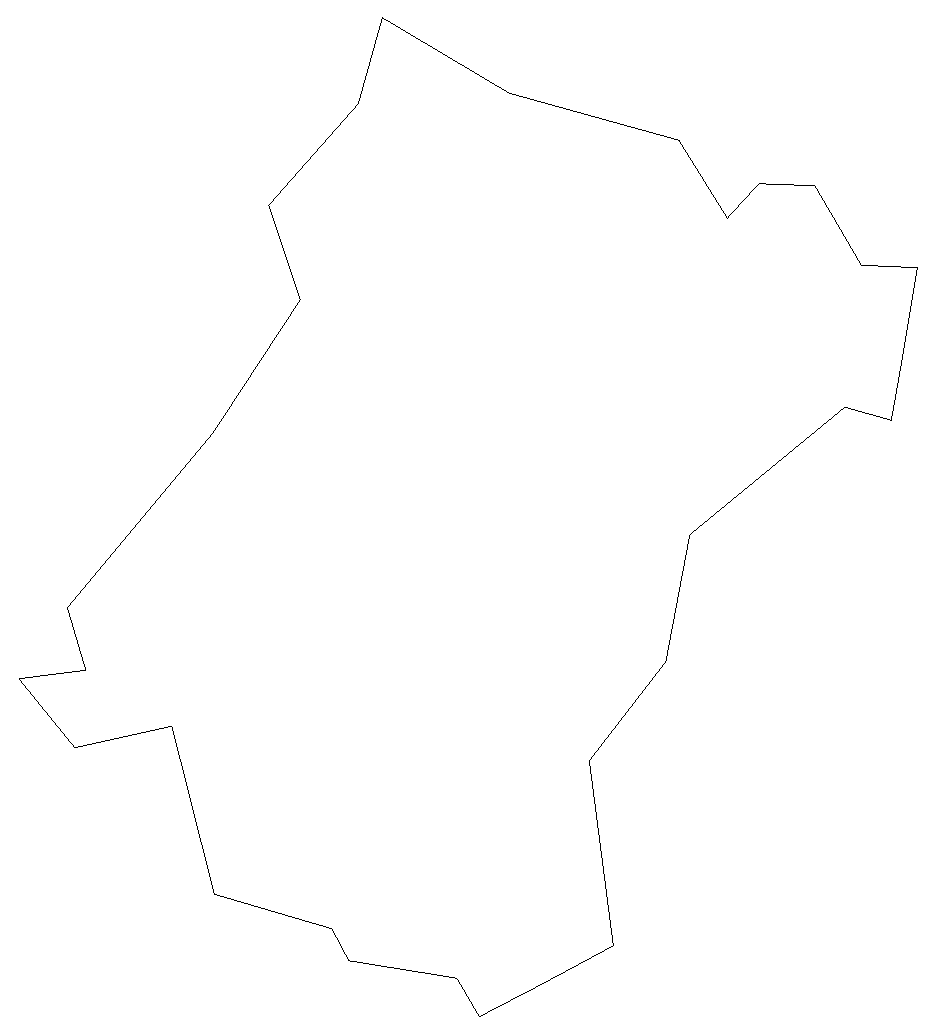
\includegraphics [scale=0.3]{grafiken/westpart.eps}
{\em\caption{\label{partgermany} Corresponding graph of the section of the boundary file}}
\end{figure}

In some cases, a region may be divided into a number of subregions that are not connected. As an example, \autoref{westsub} shows a region within Germany that is separated into 8 subregions. In such a case each subregion has to be included separately in the {\em boundary file} but all subregions should share the same region code. Note that the subregions can be placed anywhere in the {\em boundary file} and, in particular, do not have to follow each other.

Another special case that requires additional attention is illustrated in \autoref{westin}: A region is completely surrounded by another region. In this case an additional line has to be added to the boundary description of the {\em surrounded} region. This additional line is placed between the first line and the polygons and has to contain the region code of the {\em surrounding} region. The full syntax is:

#is.in#,"{\em region code}"

The following lines show a section of the {\em boundary file} of Germany, where region "9361" is totally surrounded by region "9371":

\footnotesize

\hspace{1cm} $\vdots$

"9361",7 \\
is.in,"9371" \\
4155.84668,2409.58496 \\
4161.69922,2449.38330 \\
4201.49756,2461.08862 \\
4224.90820,2478.64673 \\
4250.66016,2418.94922 \\
4193.30371,2387.34448 \\
4155.84668,2409.58496

\hspace{1cm} $\vdots$

\normalsize

\begin{figure}[hb]
\centering
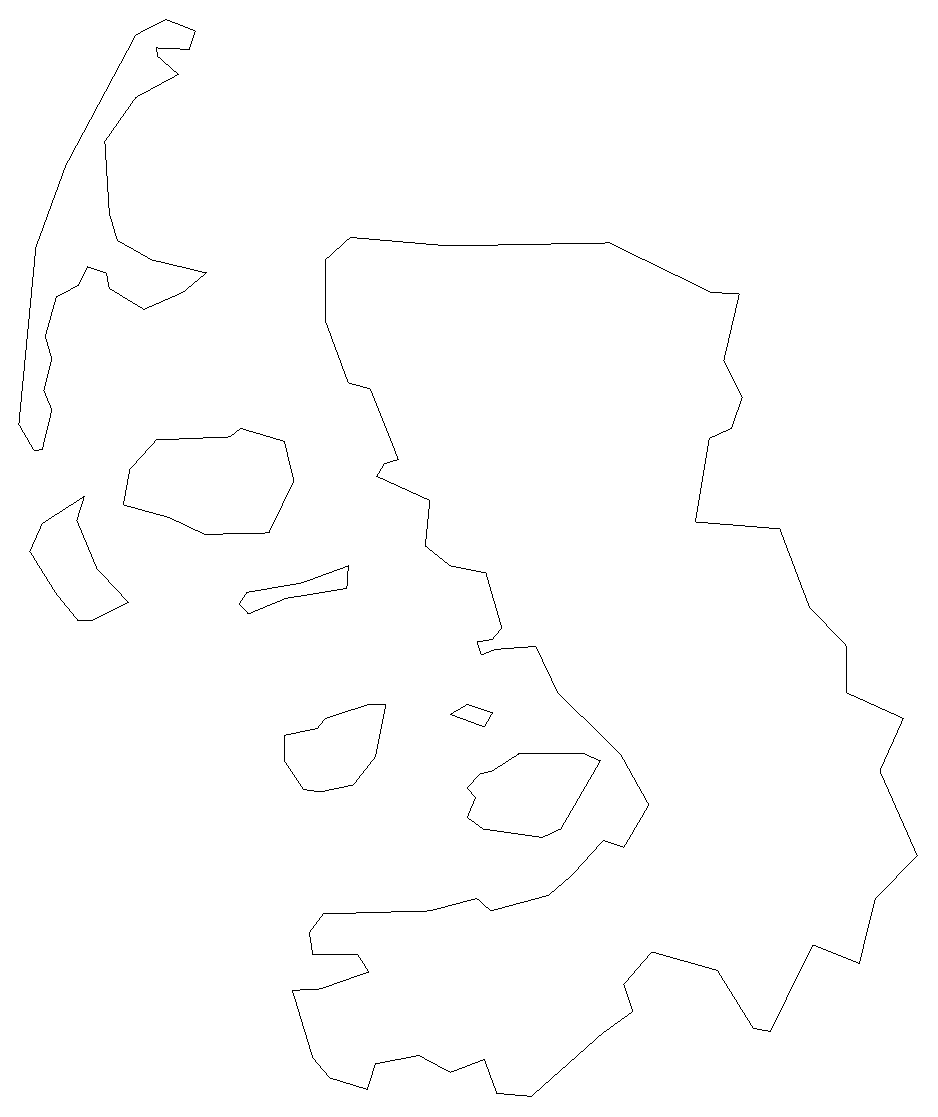
\includegraphics [scale=0.3]{grafiken/reg1054.eps}
{\em\caption{\label{westsub} Example for a region that is divided
into subregions.}}
\end{figure}

\begin{figure}[hb]
\centering
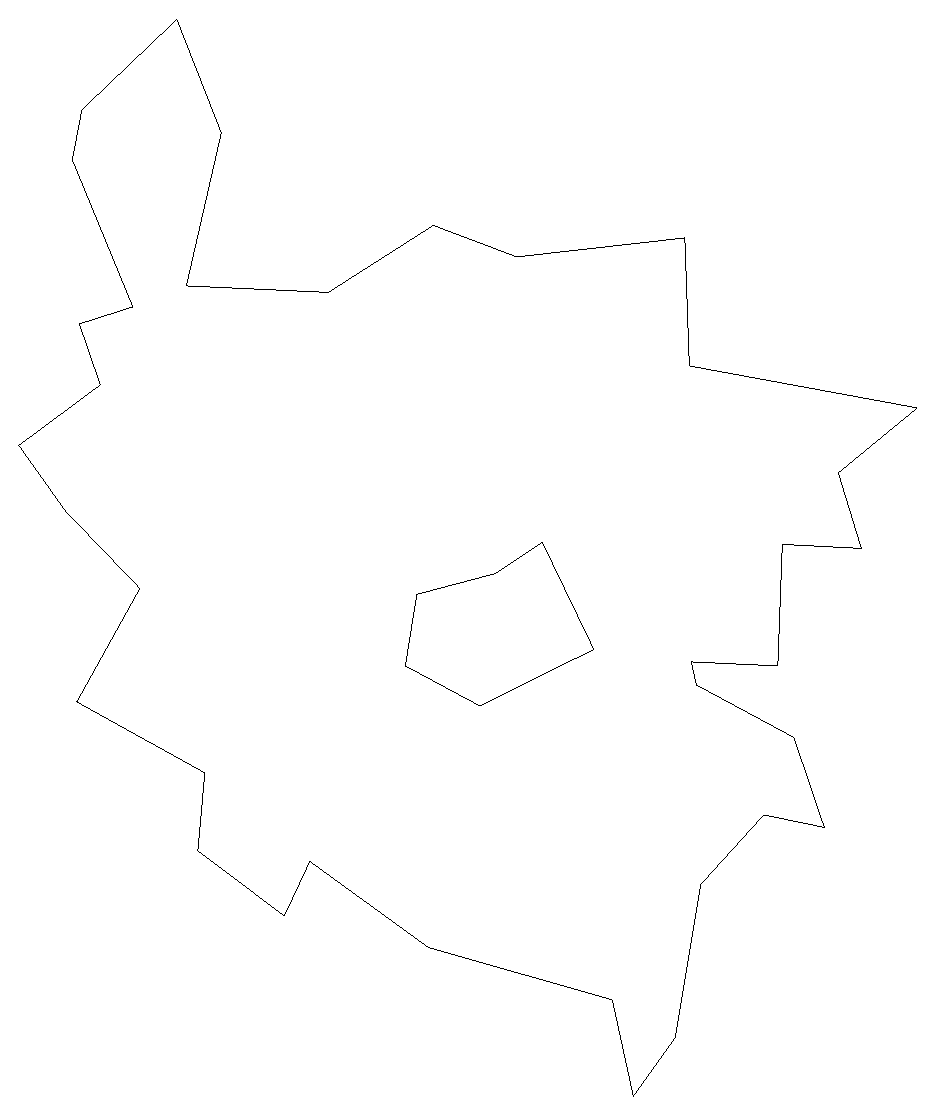
\includegraphics [scale=0.3]{grafiken/westin.eps}
{\em\caption{\label{westin} Example for a region that is totally
surrounded by another region.}}
\end{figure}

Finally, we want to draw attention to an important limitation of the current version of \BayesX. In most cases {\em map
objects} serve as auxiliary objects to estimate spatial effects with {\em bayesreg objects} or {\em remlreg objects}. In this case the names of the regions of the map and the values of the corresponding spatial covariate have to match. Since only numerical variables allowed in {\em dataset objects}, the names of the regions in the {\em map object} have to be numbers, although, in principle, there is no limitation for the names of regions in {\em map objects}.

\subsubsection*{Structure of a Graph File}

A graph file stores the nodes and the edges of a graph $G = (N,E)$, see for example \citeasnoun[Ch.~3]{GeoLiu81} for a brief introduction to graph theory. A graph is a convenient way to represent the neighborhood structure of a geographical map, where the nodes of the graph correspond to the region codes while the neighborhood structure is represented by the edges of the graph. In some situations, it can be useful to define weights associated with the edges of a graph which can be stored in the {\em graph file} as well.

In \BayesX, the first line of a {\em graph file} has to contain the total number of nodes of the graph. Afterwards, each
region (or node) is represented by a block of three lines. The first of these lines contains the name of the node (typically the name of the geographical region). The second line states the number of edges for that particular node. The third line contains the corresponding edges of the node, represented by the index of a neighboring node. Note that the index starts with zero, i.e. the first node is represented by the index 0, the second node by the index 1, and so on.

We illustrate the structure of a {\em graph file} with an example. The following few lines are the beginning of the {\em graph file} corresponding to the map of (former) West Germany:

\footnotesize

327 \\
9162 \\
3 \\
1 2 3 \\
9174 \\
6 \\
0 4 2 3 5 6 \\
9179 \\
6 \\
0 1 7 3 8 6

\hspace{1cm} $\vdots$

\normalsize

\vspace{0.5cm}

The first line specifies the total number of nodes, 327 in the present example. The subsequent three lines correspond to the node with name '9162', which is the first region in the map of West Germany. Region '9162' has 3 neighbors, namely the second, third and fourth node appearing in the graph file. Once again, note that the index starts with zero, i.e. 0 corresponds to the first node, 1 corresponds to the second node and so on. Lines 5 to 7 in the example correspond to node '9174' and its neighbors and lines 8 to 10 correspond to node '9179'.

{\em Graph files} also allow to specify weights associated with the edges of the nodes. Since no weights have been explicitly specified in the preceding example, all weights are automatically defined to be equal to one. Nonequal weights can specified in the {\em graph file} by adding them following the edges of a particular node. An example of the beginning of a {\em graph file} with weights is given below:

\footnotesize

327 \\
9162 \\
3 \\
1 2 3 0.4 1.2 0.7\\
9174 \\
6 \\
0 4 2 3 5 6 0.4 0.3 0.8 0.8 1.4 1.6\\
9179 \\
6 \\
0 1 7 3 8 6 1.2 0.8 0.2 1.8 1.7 1.3

\hspace{1cm} $\vdots$

\normalsize

\vspace{0.5cm}

In this case, the edges of the first node '9162' have weights 0.4, 1.2 and 0.7.\bigskip


\subheader{Options}
\begin{itemize}
\item #graph# \\
If #graph# is specified as an additional option, \BayesX expects a {\em graph file} rather than a {\em boundary file}.

\item #weightdef=adjacency# $|$ #centroid#  $|$ #combnd# \label{weightsmap}\\
Option #weightdef# allows to request the computation of weights associated with each pair of neighbors. Currently there are three weight specifications available: #weightdef=adjacency#, #weightdef=centroid# and #weightdef=combnd#. For #weightdef=adjacency# all weights are set equal to one. This is the most common choice in spatial statistics and also the default weight method.

Specifying #weightdef=centroid# results in weights which are inverse proportional to the distance of the centroids of
neighboring regions. More specifically, the weight $w_{us}$ of two neighboring regions $u$ and $s$ is set to $w_{us} = c \cdot \exp(-d(u,s))$, where $d$ is the Euclidian distance between the centroids of the two sites and $c$ is a normalizing constant. In analogy to adjacency weights, the constant $c$ is chosen in such a way that the total sum of weights is equal to the total number of neighbors.

The third choice #weightdef=combnd# results in weights proportional to the length of the common boundary of two regions.
Similarly to #weightdef=centroid#, the weights are normalized, i.e. the total sum of weights is equal to the number of neighbors.

Note that the specification of the #weightdef# option is only meaningful if a {\em boundary file} is read. For {\em graph files} the option has no effect since the boundary information of regions is missing and the computation of weights is therefore not possible.
\end{itemize}


\section{Method outfile}
 \label{mapoutfile} 
 \index{Map object!Outfile command}

\begin{stanza}{Description}
Method #outfile# performs the reverse of the #infile# command, i.e. the current map information is written to an external file. The map information can be written either in {\em boundary file} or in {\em graph file} format.
\end{stanza}

\begin{stanza}{Syntax}
#># {\em objectname}.#outfile# [{\em , options}] #using# {\em filename}

#outfile# writes the map information to the external file specified in {\em filename}. If #graph# is specified as an
additional option, the file format will be a {\em graph file} and a {\em boundary file} otherwise.
\end{stanza}

\subheader{Options}
\begin{itemize}
\item #graph# \\
Forces the program to store the map information in {\em graph file} format rather than in {\em boundary file} format.
\item #includeweights# \\
Option #includeweights# is meaningful only if the storing format is a {\em graph file}, i.e. if option #graph# is specified. In this case, the weights associated with the edges (neighbors) of the nodes (regions) are stored in addition to the graph structure. 
\item #replace# \\
The #replace# option allows \BayesX to overwrite an already existing file. If #replace# is omitted in the optionlist an error will be raised if you attempt to overwrite an existing file. This prevents you from overwriting an existing file unintentionally.
\end{itemize}


\section{Method reorder}
 \label{mapreorder} 
 \index{Reorder regions of a map} 
 \index{Map object!Reorder command}

\begin{stanza}{Description}
Method #reorder# reorders the regions of a map to obtain an adjacency matrix with minimal envelope. A new map should always be reordered before using it with {\em mcmcreg objects} since MCMC updates for spatial covariates will be much faster with an optimised envelope. \BayesX uses the reverse Cuthill Mc-Kee algorithm to reorder maps, see \citeasnoun[p.~58ff]{GeoLiu81}.
\end{stanza}

\begin{stanza}{Syntax}
#># {\em objectname}.#reorder#

#reorder# reorders the regions of a map in order to obtain the smallest envelope of the corresponding adjacency matrix.
\end{stanza}

\begin{stanza}{Options}
not allowed
\end{stanza}
